\chapter{Fair Matching} \label{chap:fair_matching}
    
    Matching in bipartite graphs refers to determining optimal combinations between elements of two sets, $U$ and $V$, often considering predefined constraints and specific preferences. 
    %
    This paradigm is frequently applied in contexts such as resource allocation, network design, and matching in distributed systems, which demonstrates its versatility by offering solutions to a wide range of practical problems \cite{Karp1972}.
    %
    
    %
    One of the conventional approaches to solving bipartite matching relies on reducing the problem to a Minimum Cost Max Flow (MCMF) problem, where several algorithms may be employed.
    %
    However, it does not often consider attributes among specific sub-sets of $U$ and $V$, which may possess distinct traits that are essential in various contexts.
    %
    Considering such sub-sets' characteristics makes the bipartite matching problem relevant to a large set of real-world applications, we call this the \emph{Fair Bipartite Matching Problem}.
    %

    %
    We focus on the \emph{minimum quota} characteristic among sub-sets.
    The \emph{minimum quota} defines the minimal amount of elements of each sub-set that must be matched.  % within the match // in the solution ....
    %
    By incorporating \emph{minimum quotas} for sub-sets, the proposed method aims for both: operational efficiency and equity in the distribution of resources among sub-sets. 
    %
    In this chapter, we present a reduction from the Fair Bipartite Matching Problem with \emph{minimum quota} to the MCMF.
    %

    %
    The practicality of this approach is evident in various scenarios where both qualitative and quantitative criteria are crucial in the pairing process. 
    A prominent example is in recruitment, where evaluating a potential employee's soft skills is as important as assessing their hard skills through objective methods like exams. 
    Another clear application is in network optimization, particularly in selecting the best data centers for different applications. 
    Factors such as backup type and location are just as important as latency in making these decisions.
    %
    
    %    
    Several works already address the concept of fairness, which has become increasingly important. However, most approaches rely on heuristic \cite{hatfield2005matching, rostami2018fairness, pappalardo2020algorithmic} or metaheuristic methods \cite{manlove2017algorithmics, yan2021metaheuristic, chapman2017matching}. Here, however, we develop and present a deterministic model in polynomial time, introducing an innovative approach for solving the Fair Bipartite Matching problem. The central proposal involves applying the concept of Minimum-Cost Maximum Flow (MCMF) through an effective mapping of the problem, allowing for the incorporation of fairness criteria, such as minimum quotas for specific sets.
    %

    \section{Related Works}
        Several methods have been proposed to address problems of matching and fair allocation. Table~\ref{tab:related_work} summarizes some of the most relevant approaches in terms of accuracy, fairness, and the use of minimum quotas.
        
        \begin{table}[ht]
          \centering
          \begin{tabular}{lccc}
            \toprule
            Methods & Exact & Fair & Minimum Quotas \\
            \midrule
            \textbf{Proposed} & \textbf{Yes} & \textbf{Yes} & \textbf{Yes} \\
            \cite{ahuja1993network}; \cite{edmonds1972theoretical}; \cite{tarjan1997dynamic} & Yes & No & No \\
            \cite{hatfield2005matching}; \cite{rostami2018matching}; \cite{pappalardo2020combining}; \cite{manlove2017algorithmics}; \cite{yan2021evolutionary}; \cite{chapman2017multi} & No & Yes & No \\
            \cite{sankar2021set} & No & Yes & Yes \\
            \cite{garcia2020fair} & Yes & Yes & No \\
            \bottomrule
          \end{tabular}
          \caption{Comparison of Allocation Methods, proposed and from literature, in Terms of Accuracy, Fairness, and Minimum Quotas.}
          \label{tab:related_work}
        \end{table}
        
        The methods proposed by Ahuja et al. (1993) \cite{ahuja1993network}, Edmonds and Karp (1972) \cite{Karp1972}, and Tarjan (1997) \cite{tarjan1997dynamic} focus primarily on matching accuracy without considering fairness or specific quotas.
        
        On the other hand, Hatfield and Milgrom (2005) \cite{hatfield2005matching}, Rostami et al. (2018) \cite{rostami2018matching}, Pappalardo and Conitzer (2020) \cite{pappalardo2020combining}, Manlove (2017) \cite{manlove2017algorithmics}, Yan et al. (2021) \cite{yan2021evolutionary}, and Chapman et al. (2017) \cite{chapman2017multi} address fairness in matching but do not include specific quotas in their formulations.
        
        Sankar et al. (2021) \cite{sankar2021set} present a method that considers both fairness and minimum quotas, but without exact matching. García-Soriano and Bonchi (2020) \cite{garcia2020fair} propose an exact and fair method that does not incorporate quotas.
        
        Our method proposes an approach that is exact, fair, and respects minimum quotas, promoting efficient and equitable allocation, inspired by the fairness set concept as proposed by Sankar et al. (2021) \cite{sankar2021set}.

        
        \section{Solution Modeling}
        
            As discussed in Section {\ref{subsubsec:resolucao-fluxo-matching}}, the MCMF algorithm is traditionally employed to solve matching problems without considering the concept of fairness. We present how to extend the use of MCMF to the proposed concept of fairness. This extension will be achieved through a mapping that constructs a graph to be processed by an MCMF algorithm to solve the original problem.
            
            \subsection{Objective}
            
                Based on the intrinsic characteristics of the MCMF, this method aims to maximize the flow, and among all maximum flows, select the one with the minimum cost.
                %
                In our case, we search for maximum flow to ensure fair selection in the matching, with the guarantee of respecting the predefined minimum quotas. In situations where there are multiple ways to achieve this allocation, our aim is to minimize the associated matching costs.
                
                The solution aims to meet the following points:
                
                \begin{enumerate} \item \textbf{Comply for Minimum Quotas}: Ensure that the predefined minimum quotas for all subsets are fully fulfill (if possible) during the matching process, promoting equity and inclusion. \item \textbf{Cost Minimization}: In situations where there are various matching alternatives, the objective is to minimize the costs associated with these matchings, providing operational and economic efficiency. \end{enumerate}
        
        
        \section{Modifications to Include Fairness in Bipartite Matching}
        
            The fundamental changes made to the mapping aim to make it impossible for the flow to avoid paths with minimum quota elements (in other words, to force the flow through paths with minimum quota elements), as well as to prevent the repeated selection of the same element.
            Subsequently, the reduction of the Fair Matching problem to MCMF is addressed, along with the proofs of the modeling.
            
            \subsection{Minimum Quotas}
            
                The sets of minimum quota members are defined as subsets of vertices of the same class (e.g., workers) that share one or more characteristics (e.g., workers with disability) and have a minimum number of \textit{matches} if the maximum match is achieved.
                
                Each set of minimum quota members is represented by a vertex, where the incoming edge has a capacity equivalent to the number of \textit{matches} the set needs to obtain, with an associated cost of zero. This configuration encourages the passage of the maximum flow through this vertex, as part of the total flow is required to transit through the quota vertices.
                Considering a graph with a total possible of $N$ \textit{matches} and having $|Q|$ sets of quotas, where the \( i \)-th quota, $q_i$ has $n_{q_i}$ slots.
                In Equation \ref{eq:quota_sum} we define the total matches assigned to quota slots, $N_Q$ as:

                \begin{equation}
                    N_Q = \sum_{i=1}^{|Q|} n_{q_i} \leq N
                    \label{eq:quota_sum}
                \end{equation}
                
                Thus, a set with $n_{q_i}$ quota, with the described mapping, ensures that the other vertices can only contribute a maximum of $N - N_Q$ flow units. This guarantees that if there is a maximum flow passing through the quota set, it will be selected.
                %
                In Figures~\ref{fig:mapeamento}~and~\ref{fig:solucao}, these vertices are shown in purple / loosely dash-dotted.
                
                Here, \( N \) represents the total number of possible matches, typically defined by the smaller of the two sets (demand or supply). In our case, demand (\( V \)) is always less than or equal to supply (\( U \)), so \( N \) is at most the size of the demand set \( V \). However, depending on the graph's structure and quota requirements, it is possible that not all demand is matched, meaning \( N \) can be equal to or less than \( V \).
        
        
            \subsection{Wide Competition (WC)} \label{sec:wc}
            
                The Wide Competition (WC) indicates the number of \textit{matches} that have not been previously assigned to any quota set. Let $N$ be the total possible matches overall, and $N_q$ the total matching assigned to quota slots. The wide competition slots, $n_{wc}$, is defined by Equation \ref{eq:n_wc}.
                \begin{equation}
                    n_{wc} =
                    \begin{cases}
                        N - N_Q & \text{if } N > N_Q \\
                        0 & \text{otherwise}
                    \end{cases}
                    \label{eq:n_wc}
                \end{equation}
                
                Without loss of generality, the WC set can be understood as a quota. All elements are part of the wide competition. This configuration ensures that there will be no shortage of matches if the maximum matching is possible. In Figures~\ref{fig:mapeamento} and~\ref{fig:solucao}, this vertex is represented in gray.
            
            \subsection{Proxies}
            
                A proxy is an entity represented by a vertex, whose outgoing edge has unit capacity.
                %
                There is always a proxy at the entrance of each element of the set where quotas are applied.
                %
                This proxy ensures that each element is selected only once when it participates in multiple quota groups (e.g., a worker that belongs to both, disable and female subsets, or a worker that belongs to both, WC and quota group). In Figures~\ref{fig:mapeamento} and~\ref{fig:solucao}, this vertex is identified in dark green / dash-dotted.
            
            \subsection{Mapping}
            
            For a more formal description of the mapping, consider two sets $U$ and $V$. The goal is to perform a matching $M$ between $U$ and $V$, minimizing the sum of the costs of the edges in $M$. Additionally, there is a set of quotas $Q$ of arbitrary size $|Q|$, each quota is identified by $q_i$, where $0 < i \leq |Q|$. Each quota $q_i$ represents the elements of a specific subset of $U$ (the elements that belong to the $q_i$ quota group, namely $U_{q_i}$). Each quota has an assigned number $n_{q_i}$ that represents how many elements of $q_i$ should be in the final matching. Each element of $U$, denoted as $u_i$, has its own proxy, called $p_{i}$. The set of all proxies is denoted by $P$, and a subset $P_{U_{q_i}}$ represents all proxies of the elements of $U$ that belong to quota $q_i$.
            
            The mapping always results in a multilayer graph containing six layers:
            
            \begin{itemize}
                \item \textbf{Relations between Layer 1 (\textit{Source}) and Layer 2}: The flow always originates from the \textit{Source}, located in Layer 1. It has $|Q|+1$ outgoing edges, connecting to the vertices of Layer 2, which represent each quota in $Q$ and also the \textit{wide competition} vertex, called $wc$. The weights of these edges are always zero, while the capacity is defined as $n_{q_i}$ when connected to a $q_i$ or $n_{wc}$ (number of remaining matchings) when connected to $wc$.
                
                \item \textbf{Relations between Layer 2 and Layer 3}: In Layer 3 are the proxies. Each vertex in Layer 2, $q_i$ or $wc$, has an edge with capacity 1 and cost 0 connecting it to the corresponding proxy of the element of $U$ contained in its subset. That is, every edge $q_i$ will have an edge to the elements of $P_{U_{q_i}}$. Additionally, the vertex $wc$ is connected to all vertices in Layer 3, always with capacity 1 and cost 0.
                
                \item \textbf{Relations between Layer 3 and Layer 4}: This pair of layers aims to prevent an element of $U$ from being matched more than once. Every vertex $P_{u_i}$ connects to its corresponding $u_i$, with zero cost and unit capacity.
                
                \item \textbf{Relations between Layer 4 and Layer 5}: At this stage, matching costs are taken into account. The cost of the edges connecting the two sets is defined by the relationships between elements of $U$ (Layer 4) and $V$ (Layer 5), and the cost between element $u_i$ and $v_j$ is called $C_{u_i v_j}$. Additionally, the capacity remains 1.
                
                \item \textbf{Relations between Layer 5 and Layer 6 (\textit{Sync})}: These are the final edges and serve to ensure that the elements of $V$ are matched only once, as well as to close the circuit cycle. Each element of $V$ has an edge to the \textit{Sink}, with capacity 1 and cost 0.
            \end{itemize}
            
            In Figure \ref{fig:mapeamento}, a visual representation of this mapping can be seen. Additionally, Figure \ref{fig:solucao} shows the solution to the same problem as Figure \ref{fig:mapeamento} if $U_1$, $U_2$ and $U_3$ belonged to Quota$_1$ and $U_5$ belonged to Quota$_2$.
            
            \begin{figure}[!ht]
                \centering
                \begin{subfigure}[!ht]{.95\textwidth}
                    \centering
                        \resizebox{0.7\textwidth}{!}{%
      \begin{tikzpicture} [xscale=0.45, yscale=1.05]
        \tikzstyle{style} = [circle, draw, ultra thick, minimum size=45pt, inner sep=0pt, text centered]
        \tikzstyle{no_border} = [circle, minimum size=45pt, inner sep=0pt, text centered, opacity=0.5]
        \tikzstyle{layerlabel}=[text width=5cm, align=center, font=\Large]

        
       \draw
        (-20.0, 7.5) node[layerlabel] (-1){Layer 1}
        (-12.0, 7.5) node[layerlabel] (-1){Layer 2}
        (-4.0, 7.5) node[layerlabel] (-1){Layer 3}
        (4.0, 7.5) node[layerlabel] (-1){Layer 4}
        (12.0, 7.5) node[layerlabel] (-1){Layer 5}
        (20.0, 7.5) node[layerlabel] (-1){Layer 6}
        
        (-20.0, 0.0) node[draw=black,style] (0){Source}
        (-12.0, 2.0) node[draw=purple, loosely dashdotted,style] (1){$q_1$}
        (-12.0, 0.0) node[draw=purple, loosely dashdotted,style] (2){$q_2$}
        (-12.0, -2.0) node[draw=lightgray,loosely dotted,style] (3){$wc$}
        (4.0, 5.0) node[draw=red, dashed,style] (4){$u_1$}
        (4.0, 3.0) node[draw=red, dashed,style] (5){$u_2$}
        (4.0, 1.0) node[draw=red, dashed,style] (6){$u_3$}
        (4.0, -1.0) node[draw=red, dashed,style] (7){$u_4$}
        (4.0, -3.0) node[draw=red, dashed,style] (8){$u_5$}
        (4.0, -5.0) node[draw=red, dashed,style] (9){$u_6$}
        (-4.0, 5.0) node[draw=green!50!black, dashdotted,style] (10){$p_1$}
        (-4.0, 3.0) node[draw=green!50!black, dashdotted,style] (11){$p_2$}
        (-4.0, 1.0) node[draw=green!50!black, dashdotted,style] (12){$p_3$}
        (-4.0, -1.0) node[draw=green!50!black, dashdotted,style] (13){$p_4$}
        (-4.0, -3.0) node[draw=green!50!black, dashdotted,style] (14){$p_5$}
        (-4.0, -5.0) node[draw=green!50!black, dashdotted,style] (15){$p_6$}
        (12.0, 3.0) node[draw=blue, dotted,style] (16){$v_1$}
        (12.0, -3.0) node[draw=blue, dotted,style] (17){$v_3$}
        (12.0, 0.0) node[draw=blue, dotted,style] (18){$v_2$}
        (20.0, 0.0) node[draw=black,style] (19){Sink};
      \begin{scope}[->, >=BigLatex]
        \draw[lightgray, text=black, font=\footnotesize] (0) to node[] {$n_{q_1}$ ; 0} (1);
        \draw[lightgray, text=black, font=\footnotesize] (0) to node[] {$n_{q_2}$ ; 0} (2);
        \draw[lightgray, text=black, font=\footnotesize] (0) to node[] {$n_{WC}$ ; 0} (3);
        \draw[lightgray, text=black, font=\footnotesize] (1) to node[] {1 ; 0} (10);
        \draw[lightgray, text=black, font=\footnotesize] (1) to node[] {1 ; 0} (11);
        \draw[lightgray, text=black, font=\footnotesize] (1) to node[] {1 ; 0} (12);
        % \draw[lightgray, text=black, font=\footnotesize] (2) to node[] {1 ; 0} (13);
        \draw[lightgray, text=black, font=\footnotesize] (2) to node[] {1 ; 0} (14);
        \draw[lightgray, text=black, font=\footnotesize] (3) to node[] {1 ; 0} (10);
        \draw[lightgray, text=black, font=\footnotesize] (3) to node[] {1 ; 0} (11);
        \draw[lightgray, text=black, font=\footnotesize] (3) to node[] {1 ; 0} (12);
        \draw[lightgray, text=black, font=\footnotesize] (3) to node[] {1 ; 0} (13);
        \draw[lightgray, text=black, font=\footnotesize] (3) to node[] {1 ; 0} (15);
        \draw[lightgray, text=black, font=\footnotesize] (3) to node[] {1 ; 0} (14);
        \draw[lightgray, text=black, font=\footnotesize] (10) to node[] {1 ; 0} (4);
        \draw[lightgray, text=black, font=\footnotesize] (4) to node[] {1 ; $C_{u_1 v_1}$} (16);
        \draw[lightgray, text=black, font=\footnotesize] (11) to node[] {1 ; 0} (5);
        \draw[lightgray, text=black, font=\footnotesize] (5) to node[] {1 ; $C_{u_2 v_2}$} (18);
        \draw[lightgray, text=black, font=\footnotesize] (12) to node[] {1 ; 0} (6);
        \draw[lightgray, text=black, font=\footnotesize] (6) to node[] {1 ; $C_{u_3 v_2}$} (18);
        \draw[lightgray, text=black, font=\footnotesize] (13) to node[] {1 ; 0} (7);
        \draw[lightgray, text=black, font=\footnotesize] (7) to node[] {1 ; $C_{u_4 v_3}$} (17);
        \draw[lightgray, text=black, font=\footnotesize] (15) to node[] {1 ; 0} (9);
        \draw[lightgray, text=black, font=\footnotesize] (8) to node[] {1 ; $C_{u_5 v_2}$} (18);
        \draw[lightgray, text=black, font=\footnotesize] (8) to node[] {1 ; $C_{u_5 v_3}$} (17);
        \draw[lightgray, text=black, font=\footnotesize] (14) to node[] {1 ; 0} (8);
        \draw[lightgray, text=black, font=\footnotesize] (9) to node[] {1 ; $C_{u_6 v_1}$} (16);
        \draw[lightgray, text=black, font=\footnotesize] (16) to node[] {1 ; 0} (19);
        \draw[lightgray, text=black, font=\footnotesize] (17) to node[] {1 ; 0} (19);
        \draw[lightgray, text=black, font=\footnotesize] (18) to node[] {1 ; 0} (19);
      \end{scope}
    \end{tikzpicture}
    }%

                    \caption{Example of a possible mapping of Fair Bipartite Matching.}
                    \label{fig:mapeamento}
                \end{subfigure}
                \hfill
                \begin{subfigure}[!ht]{0.8\textwidth}
                    \centering
                    \resizebox{0.7\textwidth}{!}{%
      \begin{tikzpicture} [xscale=0.45, yscale=1.05]
        \tikzstyle{style} = [circle,ultra thick, draw, minimum size=45pt, inner sep=0pt, text centered]
        \tikzstyle{no_border} = [circle,ultra thick, minimum size=45pt, inner sep=0pt, text centered, opacity=0.5]
      \tikzstyle{WC_style} = [circle,ultra thick, draw, minimum size=45pt, inner sep=0pt, text centered, text width=1.5cm, align=center, font=\scriptsize]


       \draw
        (-20.0, 0.0) node[draw=black,style] (0){Source}
        (-12.0, 2.0) node[draw=purple, loosely dashdotted,style] (1){$q$$_1$}
        (-12.0, 0.0) node[draw=purple, loosely dashdotted,style] (2){$q$$_2$}
        (-12.0, -3.0) node[draw=lightgray,loosely dotted,style] (3){$wc$}
        (4.0, 5.0) node[draw=red, dashed,,style] (4){$u$$_1$}
        (4.0, 3.0) node[draw=red, dashed,,no_border] (5){$u$$_2$}
        (4.0, 1.0) node[draw=red, dashed,,no_border] (6){$u$$_3$}
        (4.0, -1.0) node[draw=red, dashed,,style] (7){$u$$_4$}
        (4.0, -5.0) node[draw=red, dashed,,no_border] (8){$u$$_6$}
        (4.0, -3.0) node[draw=red, dashed,,style] (9){$u$$_5$}
        (-4.0, 5.0) node[draw=green!50!black, dashdotted,style] (10){$p$$_1$}
        (-4.0, 3.0) node[draw=green!50!black, dashdotted,no_border] (11){$p$$_2$}
        (-4.0, 1.0) node[draw=green!50!black, dashdotted,no_border] (12){$p$$_3$}
        (-4.0, -1.0) node[draw=green!50!black, dashdotted,style] (13){$p$$_4$}
        (-4.0, -3.0) node[draw=green!50!black, dashdotted,style] (14){$p$$_5$}
        (-4.0, -5.0) node[draw=green!50!black, dashdotted,no_border] (15){$p$$_6$}
        (12.0, 2.0) node[draw=blue, dotted,style] (16){$v$$_1$}
        (12.0, -3.0) node[draw=blue, dotted,style] (17){$v$$_3$}
        (12.0, 0.0) node[draw=blue, dotted,style] (18){$v$$_2$}
        (20.0, 0.0) node[draw=black,style] (19){Sink};
      \begin{scope}[->, >=BigLatex]
        \draw[lightgray, text=black, font=\footnotesize] (0) to node[] {1 ; 0} (1);
        \draw[lightgray, text=black, font=\footnotesize] (0) to node[] {1 ; 0} (2);
        \draw[lightgray, text=black, font=\footnotesize] (0) to node[] {1 ; 0} (3);
        \draw[lightgray, text=black, font=\footnotesize] (1) to node[] {1 ; 0} (10);
        \draw[transparent] (1) to node[] {1 ; 0} (11);
        \draw[transparent] (1) to node[] {0 ; 0} (12);
        \draw[transparent] (2) to node[] {0 ; 0} (13);
        \draw[lightgray, text=black, font=\footnotesize] (2) to node[] {1 ; 0} (14);
        \draw[transparent] (3) to node[] {1 ; 0} (10);
        \draw[transparent] (3) to node[] {0 ; 0} (11);
        \draw[transparent] (3) to node[] {0 ; 0} (12);
        \draw[lightgray, text=black, font=\footnotesize] (3) to node[] {1 ; 0} (13);
        \draw[transparent] (3) to node[] {0 ; 0} (15);
        \draw[transparent] (3) to node[] {0 ; 0} (14);
        \draw[lightgray, text=black, font=\footnotesize] (10) to node[] {1 ; 0} (4);
        \draw[lightgray, text=black, font=\footnotesize] (4) to node[] {1 ; 1} (16);
        \draw[transparent] (5) to node[] {1 ; 0} (11);
        \draw[transparent] (5) to node[] {1 ; 7} (18);
        \draw[transparent] (6) to node[] {0 ; 0} (12);
        \draw[transparent] (6) to node[] {0 ; 7} (18);
        \draw[lightgray, text=black, font=\footnotesize] (13) to node[] {1 ; 0} (7);
        \draw[lightgray, text=black, font=\footnotesize] (7) to node[] {1 ; 1} (17);
        \draw[transparent] (8) to node[] {0 ; 0} (15);
        \draw[transparent] (8) to node[] {0 ; 10} (18);
        \draw[transparent] (8) to node[] {0 ; 10} (17);
        \draw[lightgray, text=black, font=\footnotesize] (14) to node[] {1 ; 0} (9);
        \draw[lightgray, text=black, font=\footnotesize] (9) to node[] {1 ; 10} (18);
        \draw[lightgray, text=black, font=\footnotesize] (16) to node[] {1 ; 0} (19);
        \draw[lightgray, text=black, font=\footnotesize] (17) to node[] {1 ; 0} (19);
        \draw[lightgray, text=black, font=\footnotesize] (18) to node[] {1 ; 0} (19);
      \end{scope}
    \end{tikzpicture}
    }%
                    \caption[Solution of the problem from Figure \ref{fig:mapeamento}]{Solution of the problem from Figure \ref{fig:mapeamento} if $u_1$, $u_2$, and $u_3$ belonged to quota $q_1$ and $u_5$ belonged to quota $q_2$. The selected elements are those whose edge flows are not 0. The unselected elements are faded out. Total cost of 12.}
                    \label{fig:solucao}
                \end{subfigure}
                \caption{Examples of Fair Bipartite Matching mapping and its solution.}
                \label{fig:matching_examples}
            \end{figure}
        
        \section{Proofs}
        
        The objective of this proof is to demonstrate that the optimization respects the minimum quotas and minimizes costs, as well as to show that elements of a quota can participate in wide competition if it optimizes the matching.
        
        \subsection{Respecting Minimum Quotas}
        
        \begin{lemma}
           The total amount of flow passing through the vertices representing a quota $q_i$ will not exceed $n_{q_i}$.
        \end{lemma}
        
        To ensure that the predefined minimum quotas for the sets are fully respected during the matching process, it is crucial that the capacity configuration is well-defined. Each vertex in Layer 2 (quotas $q_i$ and wide competition $wc$) is connected to the \textit{Source} vertex with capacities defined as $n_{q_i}$ for $q_i$ and $n_{wc}$ for $wc$. This guarantees that the maximum number of flows for each $q_i$ is $n_{q_i}$, respecting the minimum quotas.
        
        Furthermore, the MCMF problem finds the maximum flow that passes through the graph while respecting the edge capacities. The total amount of flow passing through the vertices representing the quotas $q_i$ will not exceed $n_{q_i}$, ensuring that the minimum quotas are respected.
        
        \subsection{Cost Minimization}
        
        \begin{lemma}
           MCMF maximizes the flow in a graph, and among all maximum flows, it finds the one whose sum of edge costs is the smallest \cite{edmonds1972theoretical}.
        \end{lemma}
        
        \begin{lemma}
           The edges between the elements that optimize the MCMF represent the matchings between the elements of groups $U$ and $V$ \cite{edmonds1972theoretical}.
        \end{lemma}
        
        To minimize the costs associated with the matchings, the edges between the elements of $U$ and $V$ in Layers 4 and 5 have associated costs that represent the cost of matching. The MCMF algorithm minimizes the total cost of the flow by choosing the lowest-cost matchings between $U$ and $V$.
        
        Each edge between $U$ and $V$ has a capacity of 1, ensuring that each element is matched at most once. The minimization of the total cost will be based on selecting matchings that result in the lowest aggregate cost, respecting the capacity structure.
        
        \subsection{Respecting Matching Uniqueness}
        
        \begin{lemma}
           Every element in $U$ and $V$ has only one unit of outgoing flow, ensuring that no member of $U$ and $V$ is matched more than once.
        \end{lemma}
        
        Every element in $U$ has only one unit of outgoing flow, ensuring that no member of $U$ is matched more than once. The same analysis applies to the vertices in $V$.
        
        \subsection{Theorem Formulation}
        
        \begin{theorem}
        If the filling of the quotas is possible, the mapping of a fair bipartite matching problem to an MCMF problem will fulfill the quotas, respect the use of each resource, and minimize costs.
        \end{theorem}
        
        As discussed, the capacities and costs of the edges ensure that the quotas $q_i$ are respected. The MCMF algorithm minimizes the total cost of the matching by selecting the lowest-cost edges between $U$ and $V$. Additionally, no element of $U$ and $V$ will be matched more than once.
        
        \section{Examples}
        %{\color{green}
        The objective of this section is to demonstrate various contexts in which the mapping of fairness in matching to the Minimum Cost Maximum Flow (MCMF) problem can be effectively applied.
        
        For clarity and readability in the illustrations, the costs of the unsolved mappings will be suppressed.
        
        \subsection{Fairness in workers to positions allocation}
        \label{sec:workers_jobs_example}

        In the first scenario, we address the challenge of forming a diverse team where some workers have specific limitations, such as low vision or mobility. 
        The objective is to assemble the most diverse and optimal team possible, guaranteeing that workers with low vision and low mobility are selected for the team. 
        Each worker expresses their preferences for available job roles, and an objective evaluation method---such as an exam---assigns costs based on prior performance, with lower costs corresponding to higher performance to maintain a minimum-cost solution. Given that the jobs differ in nature, the evaluation process assigns distinct costs to each job-choice vertex, reflecting each worker's suitability for those roles.
        
        \begin{figure}[]
            \centering
            \begin{subfigure}[t]{0.8\textwidth}
                \centering
                \resizebox{0.7\textwidth}{!}{%
  \begin{tikzpicture} [xscale=0.45, yscale=1.05]
    \tikzstyle{style} = [circle, draw, ultra thick, minimum size=45pt, inner sep=0pt, text centered]
    \tikzstyle{no_border} = [circle, ultra thick, minimum size=45pt, inner sep=0pt, text centered, opacity=0.5]

    \draw
      (-20.0, 0.0) node[draw=black,style] (0){Source}
      (-12.0, 2.5) node[draw=purple, loosely dashdotted, style, text width=1.5cm, align=center] (1){$people$ $with$ $low$ \\ $vision$}
      (-12.0, 0.0) node[draw=purple, loosely dashdotted, style, text width=1.5cm, align=center] (2){$people$ $with$ $low$ \\ $mobility$}
      (-12.0, -2.5) node[draw=lightgray, loosely dotted,style] (3){$wc$}
      (4.0, 5.0) node[draw=red, dashed,style] (4){$worker_1$}
      (4.0, 3.0) node[draw=red, dashed,style] (5){$worker_2$}
      (4.0, 1.0) node[draw=red, dashed,style] (6){$worker_3$}
      (4.0, -1.0) node[draw=red, dashed,style] (7){$worker_4$}
      (4.0, -3.0) node[draw=red, dashed,style] (8){$worker_5$}
      (4.0, -5.0) node[draw=red, dashed,style] (9){$worker_6$}
      (-4.0, 5.0) node[draw=green!50!black, dashdotted,style] (10){$p_1$}
      (-4.0, 3.0) node[draw=green!50!black, dashdotted,style] (11){$p_2$}
      (-4.0, 1.0) node[draw=green!50!black, dashdotted,style] (12){$p_3$}
      (-4.0, -1.0) node[draw=green!50!black, dashdotted,style] (13){$p_4$}
      (-4.0, -3.0) node[draw=green!50!black, dashdotted,style] (14){$p_5$}
      (-4.0, -5.0) node[draw=green!50!black, dashdotted,style] (15){$p_6$}
      (12.0, 3.0) node[draw=blue, dotted,style] (16){$position_1$}
      (12.0, -3.0) node[draw=blue, dotted,style] (17){$position_3$}
      (12.0, 0.0) node[draw=blue, dotted,style] (18){$position_2$}
      (20.0, 0.0) node[draw=black,style] (19){Sink};

    \begin{scope}[->, >=BigLatex]
      \draw[lightgray, text=black, font=\footnotesize] (0) to node[] {$n_{PWLV}$ ; 0} (1);
      \draw[lightgray, text=black, font=\footnotesize] (0) to node[] {$n_{PWLM}$ ; 0} (2);
      \draw[lightgray, text=black, font=\footnotesize] (0) to node[] {$n_{wc}$ ; 0} (3);
      \draw[lightgray, text=black, font=\footnotesize] (1) to node[] {1 ; 0} (10);
      \draw[lightgray, text=black, font=\footnotesize] (1) to node[] {1 ; 0} (11);
      \draw[lightgray, text=black, font=\footnotesize] (1) to node[] {1 ; 0} (12);
      % Adjusted vertical spacing here
      \draw[lightgray, text=black, font=\footnotesize] (2) to node[] {1 ; 0} (13);
      \draw[lightgray, text=black, font=\footnotesize] (2) to node[] {1 ; 0} (14);
      \draw[lightgray, text=black, font=\footnotesize] (3) to node[] {1 ; 0} (10);
      \draw[lightgray, text=black, font=\footnotesize] (3) to node[] {1 ; 0} (11);
      \draw[lightgray, text=black, font=\footnotesize] (3) to node[] {1 ; 0} (12);
      \draw[lightgray, text=black, font=\footnotesize] (3) to node[] {1 ; 0} (13);
      \draw[lightgray, text=black, font=\footnotesize] (3) to node[] {1 ; 0} (15);
      \draw[lightgray, text=black, font=\footnotesize] (3) to node[] {1 ; 0} (14);
      \draw[lightgray, text=black, font=\footnotesize] (10) to node[] {1 ; 0} (4);
      \draw[lightgray, text=black, font=\footnotesize] (4) to node[] {1 ; $C_{W_1 P_1}$} (16);
      \draw[lightgray, text=black, font=\footnotesize] (11) to node[] {1 ; 0} (5);
      \draw[lightgray, text=black, font=\footnotesize] (5) to node[] {1 ; $C_{W_2 P_2}$} (18);
      \draw[lightgray, text=black, font=\footnotesize] (12) to node[] {1 ; 0} (6);
      \draw[lightgray, text=black, font=\footnotesize] (6) to node[] {1 ; $C_{W_3 P_2}$} (18);
      \draw[lightgray, text=black, font=\footnotesize] (13) to node[] {1 ; 0} (7);
      \draw[lightgray, text=black, font=\footnotesize] (7) to node[] {1 ; $C_{W_4 P_3}$} (17);
      \draw[lightgray, text=black, font=\footnotesize] (15) to node[] {1 ; 0} (9);
      \draw[lightgray, text=black, font=\footnotesize] (8) to node[] {1 ; $C_{W_5 P_2}$} (18);
      \draw[lightgray, text=black, font=\footnotesize] (8) to node[] {1 ; $C_{W_5 P_3}$} (17);
      \draw[lightgray, text=black, font=\footnotesize] (14) to node[] {1 ; 0} (8);
      \draw[lightgray, text=black, font=\footnotesize] (9) to node[] {1 ; $C_{W_6 P_1}$} (16);
      \draw[lightgray, text=black, font=\footnotesize] (16) to node[] {1 ; 0} (19);
      \draw[lightgray, text=black, font=\footnotesize] (17) to node[] {1 ; 0} (19);
      \draw[lightgray, text=black, font=\footnotesize] (18) to node[] {1 ; 0} (19);
    \end{scope}
  \end{tikzpicture}
}%

                \caption{Example of worker to positions mapping.}
                \label{fig:workers_jobs_unsolved}
            \end{subfigure}
            \vspace{1em}
            \begin{subfigure}[t]{0.8\textwidth}
                \centering
                 % \begin{tikzpicture}[scale=0.8]
 %      \draw
 %        (-9.0, 0.0) node[fill=cyan, rounded corners] (0){Source}
 %        (-5.745, 1.085) node[fill=pink, rounded corners] (1){Cota}
 %        (-5.745, 0.0) node[fill=pink, rounded corners] (2){Cota}
 %        (-5.745, -1.085) node[fill=gray, rounded corners] (3){Resto}
 %        (0.766, 0.0) node[fill=brown, rounded corners] (4){$u$}
 %        (0.766, -1.085) node[fill=brown, rounded corners] (5){$u$}
 %        (0.766, 1.085) node[fill=brown, rounded corners] (6){$u$}
 %        (-2.489, 1.085) node[fill=yellow, rounded corners] (7){$p$}
 %        (-2.489, 0.0) node[fill=yellow, rounded corners] (8){$p$}
 %        (-2.489, -1.085) node[fill=yellow, rounded corners] (9){$p$}
 %        (4.021, 2.713) node[fill=orange, rounded corners] (10){$u$}
 %        (4.021, 1.628) node[fill=orange, rounded corners] (11){$u$}
 %        (4.021, 0.543) node[fill=orange, rounded corners] (12){$u$}
 %        (4.021, -0.543) node[fill=orange, rounded corners] (13){$u$}
 %        (4.021, -1.628) node[fill=orange, rounded corners] (14){$u$}
 %        (4.021, -2.713) node[fill=orange, rounded corners] (15){$u$}
 %        (7.277, 0.0) node[fill=cyan, rounded corners] (16){Target};
 %      \begin{scope}[-]
 %        \draw[lightgray, text=black, font=\footnotesize] (0) to node[] {0} (1);
 %        \draw[lightgray, text=black, font=\footnotesize] (0) to node[] {0} (2);
 %        \draw[lightgray, text=black, font=\footnotesize] (0) to node[] {0} (3);
 %        \draw[lightgray, text=black, font=\footnotesize] (1) to node[] {0} (7);
 %        \draw[lightgray, text=black, font=\footnotesize] (2) to node[] {0} (8);
 %        \draw[transparent] (3) to node[] {0 ; 0} (8);
 %        \draw[lightgray, text=black, font=\footnotesize] (3) to node[] {0} (9);
 %        \draw[transparent] (3) to node[] {0 ; 0} (7);
 %        \draw[lightgray, text=black, font=\footnotesize] (4) to node[] {0} (8);
 %        \draw[transparent] (4) to node[] {0 ; 4} (14);
 %        \draw[lightgray, text=black, font=\footnotesize] (4) to node[] {2} (13);
 %        \draw[transparent] (4) to node[] {0 ; 5} (12);
 %        \draw[transparent] (4) to node[] {0 ; 4} (11);
 %        \draw[lightgray, text=black, font=\footnotesize] (5) to node[] {0} (9);
 %        \draw[transparent] (5) to node[] {0 ; 4} (14);
 %        \draw[transparent] (5) to node[] {0 ; 2} (13);
 %        \draw[lightgray, text=black, font=\footnotesize] (5) to node[] {2} (15);
 %        \draw[transparent] (5) to node[] {0 ; 3} (11);
 %        \draw[lightgray, text=black, font=\footnotesize] (6) to node[] {0} (7);
 %        \draw[lightgray, text=black, font=\footnotesize] (6) to node[] {1} (10);
 %        \draw[transparent] (6) to node[] {0 ; 1} (14);
 %        \draw[lightgray, text=black, font=\footnotesize] (10) to node[] {0} (16);
 %        \draw[transparent] (11) to node[] {0 ; 0} (16);
 %        \draw[transparent] (12) to node[] {0 ; 0} (16);
 %        \draw[lightgray, text=black, font=\footnotesize] (13) to node[] {0} (16);
 %        \draw[transparent] (14) to node[] {0 ; 0} (16);
 %        \draw[lightgray, text=black, font=\footnotesize] (15) to node[] {0} (16);
 %      \end{scope}
 %    \end{tikzpicture}

\resizebox{0.7\textwidth}{!}{%
      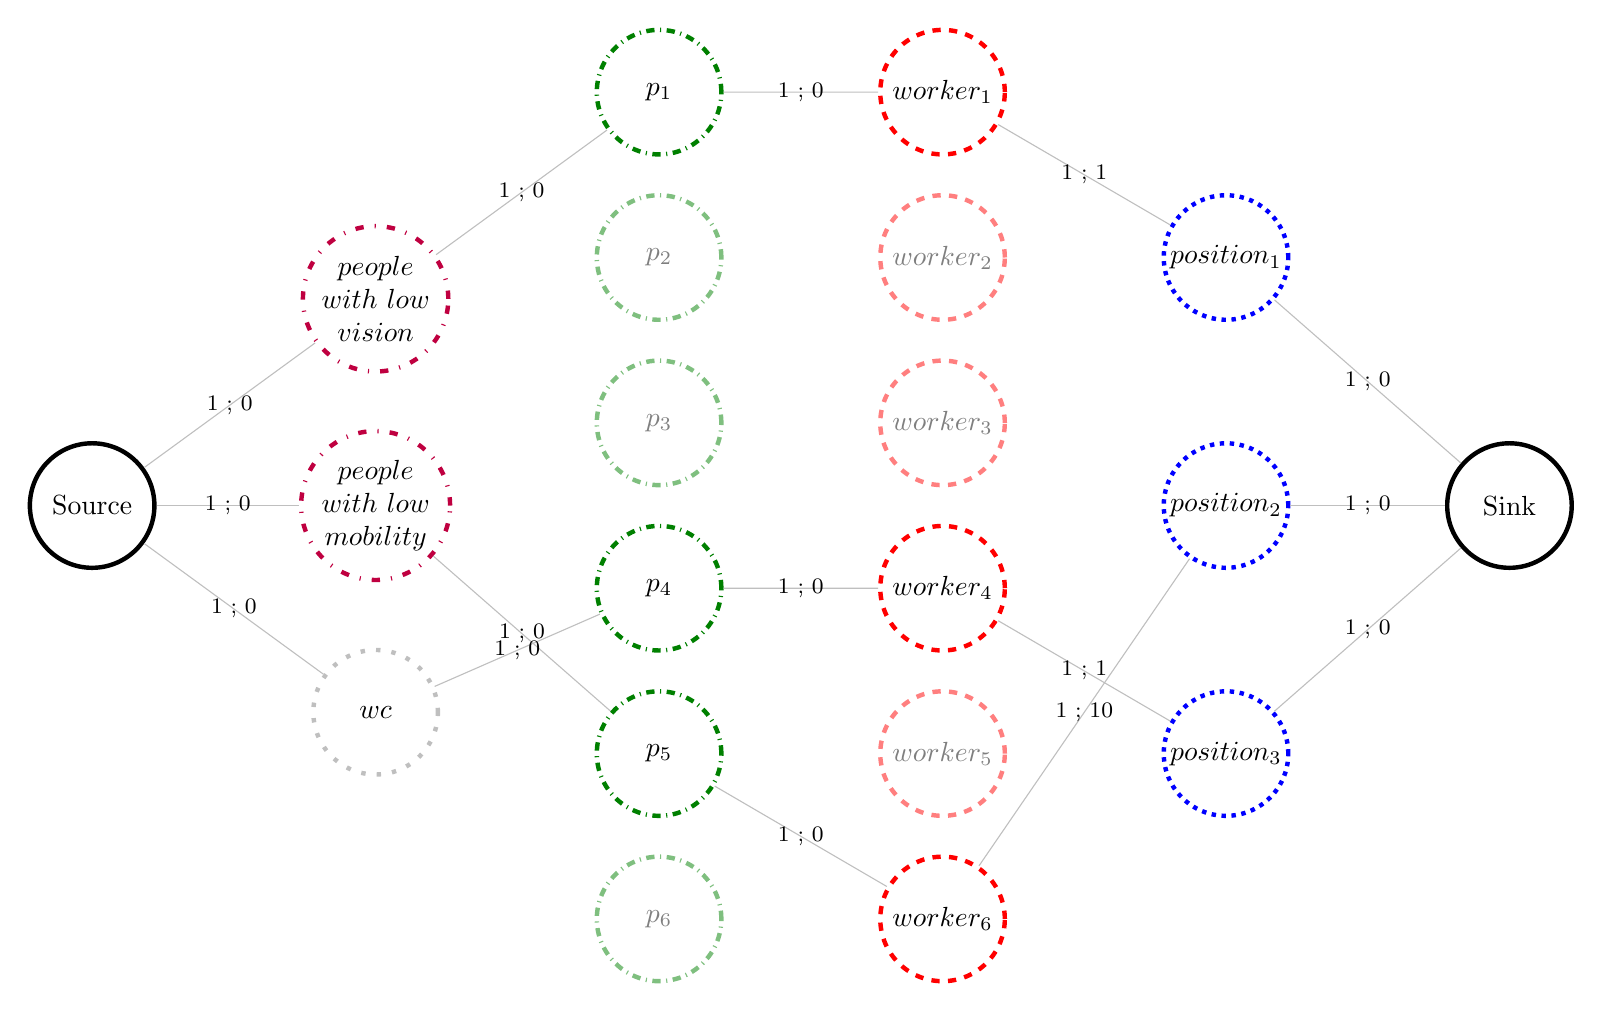
\begin{tikzpicture} [xscale=0.45, yscale=1.05]

      \tikzstyle{WC_style} = [circle, draw, fill, minimum size=45pt, inner sep=0pt, text centered, text width=1.5cm, align=center, font=\scriptsize]
        \tikzstyle{style} = [circle, draw, ultra thick, minimum size=45pt, inner sep=0pt, text centered]
            \tikzstyle{no_border} = [circle, ultra thick, minimum size=45pt, inner sep=0pt, text centered, opacity=0.5]
        
            \draw
              (-20.0, 0.0) node[draw=black,style] (0){Source}
              (-12.0, 2.5) node[draw=purple, loosely dashdotted, style, text width=1.5cm, align=center] (1){$people$ $with$ $low$ \\ $vision$}
              (-12.0, 0.0) node[draw=purple, loosely dashdotted, style, text width=1.5cm, align=center] (2){$people$ $with$ $low$ \\ $mobility$}
              (-12.0, -2.5) node[draw=lightgray, loosely dotted,style] (3){$wc$}
              (4.0, 5.0) node[draw=red, dashed,style] (4){$worker_1$}
              (4.0, 3.0) node[draw=red, dashed,no_border] (5){$worker_2$}
              (4.0, 1.0) node[draw=red, dashed,no_border] (6){$worker_3$}
              (4.0, -1.0) node[draw=red, dashed,style] (7){$worker_4$}
              (4.0, -3.0) node[draw=red, dashed,no_border] (8){$worker_5$}
              (4.0, -5.0) node[draw=red, dashed,style] (9){$worker_6$}
              (-4.0, 5.0) node[draw=green!50!black, dashdotted,style] (10){$p_1$}
              (-4.0, 3.0) node[draw=green!50!black, dashdotted,no_border] (11){$p_2$}
              (-4.0, 1.0) node[draw=green!50!black, dashdotted,no_border] (12){$p_3$}
              (-4.0, -1.0) node[draw=green!50!black, dashdotted,style] (13){$p_4$}
              (-4.0, -3.0) node[draw=green!50!black, dashdotted,style] (14){$p_5$}
              (-4.0, -5.0) node[draw=green!50!black, dashdotted,no_border] (15){$p_6$}
              (12.0, 3.0) node[draw=blue, dotted,style] (16){$position_1$}
              (12.0, -3.0) node[draw=blue, dotted,style] (17){$position_3$}
              (12.0, 0.0) node[draw=blue, dotted,style] (18){$position_2$}
              (20.0, 0.0) node[draw=black,style] (19){Sink};
        
      \begin{scope}[-]
        \draw[lightgray, text=black, font=\footnotesize] (0) to node[] {1 ; 0} (1);
        \draw[lightgray, text=black, font=\footnotesize] (0) to node[] {1 ; 0} (2);
        \draw[lightgray, text=black, font=\footnotesize] (0) to node[] {1 ; 0} (3);
        \draw[lightgray, text=black, font=\footnotesize] (1) to node[] {1 ; 0} (10);
        \draw[transparent] (1) to node[] {1 ; 0} (11);
        \draw[transparent] (1) to node[] {0 ; 0} (12);
        \draw[transparent] (2) to node[] {0 ; 0} (13);
        \draw[lightgray, text=black, font=\footnotesize] (2) to node[] {1 ; 0} (14);
        \draw[transparent] (3) to node[] {1 ; 0} (10);
        \draw[transparent] (3) to node[] {0 ; 0} (11);
        \draw[transparent] (3) to node[] {0 ; 0} (12);
        \draw[lightgray, text=black, font=\footnotesize] (3) to node[] {1 ; 0} (13);
        \draw[transparent] (3) to node[] {0 ; 0} (15);
        \draw[transparent] (3) to node[] {0 ; 0} (14);
        \draw[lightgray, text=black, font=\footnotesize] (4) to node[] {1 ; 0} (10);
        \draw[lightgray, text=black, font=\footnotesize] (4) to node[] {1 ; 1} (16);
        \draw[transparent] (5) to node[] {1 ; 0} (11);
        \draw[transparent] (5) to node[] {1 ; 7} (18);
        \draw[transparent] (6) to node[] {0 ; 0} (12);
        \draw[transparent] (6) to node[] {0 ; 7} (18);
        \draw[lightgray, text=black, font=\footnotesize] (7) to node[] {1 ; 0} (13);
        \draw[lightgray, text=black, font=\footnotesize] (7) to node[] {1 ; 1} (17);
        \draw[transparent] (8) to node[] {0 ; 0} (15);
        \draw[transparent] (8) to node[] {0 ; 10} (18);
        \draw[transparent] (8) to node[] {0 ; 10} (17);
        \draw[lightgray, text=black, font=\footnotesize] (9) to node[] {1 ; 0} (14);
        \draw[lightgray, text=black, font=\footnotesize] (9) to node[] {1 ; 10} (18);
        \draw[lightgray, text=black, font=\footnotesize] (16) to node[] {1 ; 0} (19);
        \draw[lightgray, text=black, font=\footnotesize] (17) to node[] {1 ; 0} (19);
        \draw[lightgray, text=black, font=\footnotesize] (18) to node[] {1 ; 0} (19);
      \end{scope}
    \end{tikzpicture}
    }%
                \caption[Example of a solution for mapping workers to jobs in Figure \ref{fig:workers_jobs_unsolved}.]{Example of a solution for mapping workers to jobs in Figure \ref{fig:workers_jobs_unsolved}. In this example each quota has at least one assemble. Unselected workers and their proxies are faded out.}
                \label{fig:workers_jobs_solved}
            \end{subfigure}
            \vspace{1em}
            \begin{subfigure}[t]{0.8\textwidth}
                \centering
                
\resizebox{0.7\textwidth}{!}{%
      \begin{tikzpicture} [xscale=0.45, yscale=1.05]

      \tikzstyle{WC_style} = [circle, draw, fill, minimum size=45pt, inner sep=0pt, text centered, text width=1.5cm, align=center, font=\scriptsize]
        \tikzstyle{style} = [circle, draw, ultra thick, minimum size=45pt, inner sep=0pt, text centered]
            \tikzstyle{no_border} = [circle, ultra thick, minimum size=45pt, inner sep=0pt, text centered, opacity=0.5]
        
            \draw
              (-20.0, 0.0) node[draw=black,style] (0){Source}
              (-12.0, 2.5) node[draw=purple, loosely dashdotted, style, text width=1.5cm, align=center] (1){$people$ $with$ $low$ \\ $vision$}
              (-12.0, 0.0) node[draw=purple, loosely dashdotted, style, text width=1.5cm, align=center] (2){$people$ $with$ $low$ \\ $mobility$}
              (-12.0, -2.5) node[draw=lightgray, loosely dotted,no_border] (3){$wc$}
              (4.0, 5.0) node[draw=red, dashed,style] (4){$worker_1$}
              (4.0, 3.0) node[draw=red, dashed,no_border] (5){$worker_2$}
              (4.0, 1.0) node[draw=red, dashed,no_border] (6){$worker_3$}
              (4.0, -1.0) node[draw=red, dashed,style] (7){$worker_4$}
              (4.0, -3.0) node[draw=red, dashed,no_border] (8){$worker_5$}
              (4.0, -5.0) node[draw=red, dashed,style] (9){$worker_6$}
              (-4.0, 5.0) node[draw=green!50!black, dashdotted,style] (10){$p_1$}
              (-4.0, 3.0) node[draw=green!50!black, dashdotted,no_border] (11){$p_2$}
              (-4.0, 1.0) node[draw=green!50!black, dashdotted,no_border] (12){$p_3$}
              (-4.0, -1.0) node[draw=green!50!black, dashdotted,style] (13){$p_4$}
              (-4.0, -3.0) node[draw=green!50!black, dashdotted,style] (14){$p_5$}
              (-4.0, -5.0) node[draw=green!50!black, dashdotted,no_border] (15){$p_6$}
              (12.0, 3.0) node[draw=blue, dotted,style] (16){$position_1$}
              (12.0, -3.0) node[draw=blue, dotted,style] (17){$position_3$}
              (12.0, 0.0) node[draw=blue, dotted,style] (18){$position_2$}
              (20.0, 0.0) node[draw=black,style] (19){Sink};
        
      \begin{scope}[->, >=BigLatex]
        \draw[lightgray, text=black, font=\footnotesize] (0) to node[] {1 ; 0} (1);
        \draw[lightgray, text=black, font=\footnotesize] (0) to node[] {2 ; 0} (2);
        \draw[transparent] (0) to node[] {2 ; 0} (3);
        \draw[lightgray, text=black, font=\footnotesize] (1) to node[] {1 ; 0} (10);
        \draw[transparent] (1) to node[] {1 ; 0} (11);
        \draw[transparent] (1) to node[] {0 ; 0} (12);
        \draw[transparent] (2) to node[] {0 ; 0} (13);
        \draw[transparent] (2) to node[] {1 ; 0} (14);
        \draw[transparent] (3) to node[] {1 ; 0} (10);
        \draw[transparent] (3) to node[] {0 ; 0} (11);
        \draw[transparent] (2) to node[] {1 ; 0} (12);
        \draw[lightgray, text=black, font=\footnotesize] (2) to node[] {1 ; 0} (13);
        \draw[transparent] (3) to node[] {0 ; 0} (15);
        \draw[lightgray, text=black, font=\footnotesize] (2) to node[] {1 ; 0} (14);
        \draw[lightgray, text=black, font=\footnotesize] (10) to node[] {1 ; 0} (4);
        \draw[lightgray, text=black, font=\footnotesize] (4) to node[] {1 ; 1} (16);
        \draw[transparent] (5) to node[] {1 ; 0} (11);
        \draw[transparent] (5) to node[] {1 ; 7} (18);
        \draw[transparent] (6) to node[] {0 ; 0} (12);
        \draw[transparent] (6) to node[] {0 ; 7} (18);
        \draw[lightgray, text=black, font=\footnotesize] (13) to node[] {1 ; 0} (7);
        \draw[lightgray, text=black, font=\footnotesize] (7) to node[] {1 ; 1} (17);
        \draw[transparent] (8) to node[] {0 ; 0} (15);
        \draw[transparent] (8) to node[] {0 ; 10} (18);
        \draw[transparent] (8) to node[] {0 ; 10} (17);
        \draw[lightgray, text=black, font=\footnotesize] (14) to node[] {1 ; 0} (9);
        \draw[lightgray, text=black, font=\footnotesize] (9) to node[] {1 ; 10} (18);
        \draw[lightgray, text=black, font=\footnotesize] (16) to node[] {1 ; 0} (19);
        \draw[lightgray, text=black, font=\footnotesize] (17) to node[] {1 ; 0} (19);
        \draw[lightgray, text=black, font=\footnotesize] (18) to node[] {1 ; 0} (19);
      \end{scope}
    \end{tikzpicture}
    }%
                \caption[Example of a solution for mapping workers to jobs in Figure \ref{fig:workers_jobs_unsolved}.]{Example of a solution for mapping workers to jobs in Figure \ref{fig:workers_jobs_unsolved}. In this example the `people with low mobility' quota has a minimum of 2 assembles, thus no wide competition is assembled. Unselected workers and their proxies are faded out.}
                \label{fig:workers_jobs_solved_no_wc}
            \end{subfigure}
            \caption{Examples of worker to positions mapping and their solutions. (a) shows the initial mapping, (b) presents a solution with at least one assemble per quota, and (c) shows a solution where no wide competition is assembled.}
            \label{fig:workers_jobs_example}
        \end{figure}
        
         
        The result that can be seen in Figure {\ref{fig:workers_jobs_solved}} is a minimum-cost solution that maximizes the diversity of attributes among the selected workers, ensuring both fairness and efficiency in the team formation process. 
        
        \subsection{Fairness in server to services allocation}
        
        In the second example, we address a resource allocation problem within a network of services belonging to a single application. The goal is to assign these services to servers, each of which possesses distinct attributes, such as geolocation and backup methods. The objective is to ensure the most diverse and optimal distribution of services across the available servers. An evaluation process assigns costs based on factors like latency, representing the suitability of each service-server pair. This cost structure ensures that resources are allocated in a way that balances fairness and efficiency while maximizing server characteristics that minimize overall costs.

        \begin{figure}[]
            \centering
            \begin{subfigure}[t]{0.8\textwidth}
            \centering
            \resizebox{0.7\textwidth}{!}{%
  \begin{tikzpicture} [xscale=0.45, yscale=1.05]
    \tikzstyle{style} = [circle, draw, ultra thick, minimum size=45pt, inner sep=0pt, text centered]
    \tikzstyle{no_border} = [circle, ultra thick, minimum size=45pt, inner sep=0pt, text centered, opacity=0.5]

    \draw
      (-20.0, 0.0) node[draw=black,style] (0){Source}
      (-12.0, 2.5) node[draw=purple, loosely dashdotted, style, text width=1.5cm, align=center] (1){$diverse$ $geolocation$}
      (-12.0, 0.0) node[draw=purple, loosely dashdotted, style, text width=1.5cm, align=center] (2){$robust$ $backup$}
      (-12.0, -2.5) node[draw=lightgray,loosely dotted,style] (3){$wc$}
      (4.0, 5.0) node[draw=red, dashed,style] (4){$server_1$}
      (4.0, 3.0) node[draw=red, dashed,style] (5){$server_2$}
      (4.0, 1.0) node[draw=red, dashed,style] (6){$server_3$}
      (4.0, -1.0) node[draw=red, dashed,style] (7){$server_4$}
      (4.0, -3.0) node[draw=red, dashed,style] (8){$server_5$}
      (4.0, -5.0) node[draw=red, dashed,style] (9){$server_6$}
      (-4.0, 5.0) node[draw=green!50!black, dashdotted,style] (10){$p_1$}
      (-4.0, 3.0) node[draw=green!50!black, dashdotted,style] (11){$p_2$}
      (-4.0, 1.0) node[draw=green!50!black, dashdotted,style] (12){$p_3$}
      (-4.0, -1.0) node[draw=green!50!black, dashdotted,style] (13){$p_4$}
      (-4.0, -3.0) node[draw=green!50!black, dashdotted,style] (14){$p_5$}
      (-4.0, -5.0) node[draw=green!50!black, dashdotted,style] (15){$p_6$}
      (12.0, 3.0) node[draw=blue, dotted,style] (16){$service_1$}
      (12.0, -3.0) node[draw=blue, dotted,style] (18){$service_2$}
      (20.0, 0.0) node[draw=black,style] (19){Sink};

    \begin{scope}[-]
      \draw[lightgray, text=black, font=\footnotesize] (0) to node[] {$n_{SDG}$ ; 0} (1);
      \draw[lightgray, text=black, font=\footnotesize] (0) to node[] {$n_{RB}$ ; 0} (2);
      \draw[lightgray, text=black, font=\footnotesize] (0) to node[] {$n_{wc}$ ; 0} (3);
      \draw[lightgray, text=black, font=\footnotesize] (1) to node[] {1 ; 0} (10);
      \draw[lightgray, text=black, font=\footnotesize] (1) to node[] {1 ; 0} (11);
      \draw[lightgray, text=black, font=\footnotesize] (1) to node[] {1 ; 0} (12);
      % Adjusted vertical spacing here
      \draw[lightgray, text=black, font=\footnotesize] (2) to node[] {1 ; 0} (13);
      \draw[lightgray, text=black, font=\footnotesize] (2) to node[] {1 ; 0} (14);
      \draw[lightgray, text=black, font=\footnotesize] (3) to node[] {1 ; 0} (10);
      \draw[lightgray, text=black, font=\footnotesize] (3) to node[] {1 ; 0} (11);
      \draw[lightgray, text=black, font=\footnotesize] (3) to node[] {1 ; 0} (12);
      \draw[lightgray, text=black, font=\footnotesize] (3) to node[] {1 ; 0} (13);
      \draw[lightgray, text=black, font=\footnotesize] (3) to node[] {1 ; 0} (15);
      \draw[lightgray, text=black, font=\footnotesize] (3) to node[] {1 ; 0} (14);
      \draw[lightgray, text=black, font=\footnotesize] (4) to node[] {1 ; 0} (10);
      \draw[lightgray, text=black, font=\footnotesize] (4) to node[] {1 ; $C_{SVE_1 SVI_1}$} (16);
      \draw[lightgray, text=black, font=\footnotesize] (5) to node[] {1 ; 0} (11);
      \draw[lightgray, text=black, font=\footnotesize] (5) to node[] {1 ; $C_{SVE_2 SVI_2}$} (18);
      \draw[lightgray, text=black, font=\footnotesize] (6) to node[] {1 ; 0} (12);
      \draw[lightgray, text=black, font=\footnotesize] (6) to node[] {1 ; $C_{SVE_3 SVI_2}$} (18);
      \draw[lightgray, text=black, font=\footnotesize] (7) to node[] {1 ; 0} (13);
      \draw[lightgray, text=black, font=\footnotesize] (7) to node[] {1 ; $C_{SVE_4 SVI_2}$} (18);
      \draw[lightgray, text=black, font=\footnotesize] (9) to node[] {1 ; 0} (15);
      \draw[lightgray, text=black, font=\footnotesize] (8) to node[] {1 ; $C_{SVE_5 SVI_2}$} (18);
      \draw[lightgray, text=black, font=\footnotesize] (8) to node[] {1 ; $C_{SVE_5 SVI_2}$} (18);
      \draw[lightgray, text=black, font=\footnotesize] (8) to node[] {1 ; 0} (14);
      \draw[lightgray, text=black, font=\footnotesize] (9) to node[] {1 ; $C_{SVE_6 SVI_2}$} (18);
      \draw[lightgray, text=black, font=\footnotesize] (16) to node[] {1 ; 0} (19);
      \draw[lightgray, text=black, font=\footnotesize] (17) to node[] {1 ; 0} (19);
      \draw[lightgray, text=black, font=\footnotesize] (18) to node[] {1 ; 0} (19);
    \end{scope}
  \end{tikzpicture}
}%

            \caption{Server to services mapping.}
            \label{fig:server_services_unsolved}
            \end{subfigure}
            \vspace{1em}
            \begin{subfigure}[t]{0.8\textwidth}
            \centering
             % \begin{tikzpicture}[scale=0.8]
 %      \draw
 %        (-9.0, 0.0) node[fill=cyan, rounded corners] (0){Source}
 %        (-5.745, 1.085) node[fill=pink, rounded corners] (1){Cota}
 %        (-5.745, 0.0) node[fill=pink, rounded corners] (2){Cota}
 %        (-5.745, -1.085) node[fill=gray, rounded corners] (3){Resto}
 %        (0.766, 0.0) node[fill=brown, rounded corners] (4){$u$}
 %        (0.766, -1.085) node[fill=brown, rounded corners] (5){$u$}
 %        (0.766, 1.085) node[fill=brown, rounded corners] (6){$u$}
 %        (-2.489, 1.085) node[fill=yellow, rounded corners] (7){$p$}
 %        (-2.489, 0.0) node[fill=yellow, rounded corners] (8){$p$}
 %        (-2.489, -1.085) node[fill=yellow, rounded corners] (9){$p$}
 %        (4.021, 2.713) node[fill=orange, rounded corners] (10){$u$}
 %        (4.021, 1.628) node[fill=orange, rounded corners] (11){$u$}
 %        (4.021, 0.543) node[fill=orange, rounded corners] (12){$u$}
 %        (4.021, -0.543) node[fill=orange, rounded corners] (13){$u$}
 %        (4.021, -1.628) node[fill=orange, rounded corners] (14){$u$}
 %        (4.021, -2.713) node[fill=orange, rounded corners] (15){$u$}
 %        (7.277, 0.0) node[fill=cyan, rounded corners] (16){Target};
 %      \begin{scope}[-]
 %        \draw[lightgray, text=black, font=\footnotesize] (0) to node[] {0} (1);
 %        \draw[lightgray, text=black, font=\footnotesize] (0) to node[] {0} (2);
 %        \draw[lightgray, text=black, font=\footnotesize] (0) to node[] {0} (3);
 %        \draw[lightgray, text=black, font=\footnotesize] (1) to node[] {0} (7);
 %        \draw[lightgray, text=black, font=\footnotesize] (2) to node[] {0} (8);
 %        \draw[transparent] (3) to node[] {0 ; 0} (8);
 %        \draw[lightgray, text=black, font=\footnotesize] (3) to node[] {0} (9);
 %        \draw[transparent] (3) to node[] {0 ; 0} (7);
 %        \draw[lightgray, text=black, font=\footnotesize] (4) to node[] {0} (8);
 %        \draw[transparent] (4) to node[] {0 ; 4} (14);
 %        \draw[lightgray, text=black, font=\footnotesize] (4) to node[] {2} (13);
 %        \draw[transparent] (4) to node[] {0 ; 5} (12);
 %        \draw[transparent] (4) to node[] {0 ; 4} (11);
 %        \draw[lightgray, text=black, font=\footnotesize] (5) to node[] {0} (9);
 %        \draw[transparent] (5) to node[] {0 ; 4} (14);
 %        \draw[transparent] (5) to node[] {0 ; 2} (13);
 %        \draw[lightgray, text=black, font=\footnotesize] (5) to node[] {2} (15);
 %        \draw[transparent] (5) to node[] {0 ; 3} (11);
 %        \draw[lightgray, text=black, font=\footnotesize] (6) to node[] {0} (7);
 %        \draw[lightgray, text=black, font=\footnotesize] (6) to node[] {1} (10);
 %        \draw[transparent] (6) to node[] {0 ; 1} (14);
 %        \draw[lightgray, text=black, font=\footnotesize] (10) to node[] {0} (16);
 %        \draw[transparent] (11) to node[] {0 ; 0} (16);
 %        \draw[transparent] (12) to node[] {0 ; 0} (16);
 %        \draw[lightgray, text=black, font=\footnotesize] (13) to node[] {0} (16);
 %        \draw[transparent] (14) to node[] {0 ; 0} (16);
 %        \draw[lightgray, text=black, font=\footnotesize] (15) to node[] {0} (16);
 %      \end{scope}
 %    \end{tikzpicture}

\resizebox{0.7\textwidth}{!}{%
      \begin{tikzpicture} [xscale=0.45, yscale=1.05]
        \tikzstyle{style} = [circle, draw, ultra thick, minimum size=45pt, inner sep=0pt, text centered]
    \tikzstyle{no_border} = [circle, ultra thick, minimum size=45pt, inner sep=0pt, text centered, opacity=0.5]

    \draw
      (-20.0, 0.0) node[draw=black,style] (0){Source}
      (-12.0, 2.5) node[draw=purple, loosely dashdotted, style, text width=1.5cm, align=center] (1){$diverse$ $geolocation$}
      (-12.0, 0.0) node[draw=purple, loosely dashdotted, style, text width=1.5cm, align=center] (2){$robust$ $backup$}
      (-12.0, -2.5) node[draw=lightgray,loosely dotted,no_border] (3){$wc$}
      (4.0, 5.0) node[draw=red, dashed,style] (4){$server_1$}
      (4.0, 3.0) node[draw=red, dashed,no_border] (5){$server_2$}
      (4.0, 1.0) node[draw=red, dashed,no_border] (6){$server_3$}
      (4.0, -1.0) node[draw=red, dashed,no_border] (7){$server_4$}
      (4.0, -3.0) node[draw=red, dashed,no_border] (8){$server_5$}
      (4.0, -5.0) node[draw=red, dashed,style] (9){$server_6$}
      (-4.0, 5.0) node[draw=green!50!black, dashdotted,style] (10){$p_1$}
      (-4.0, 3.0) node[draw=green!50!black, dashdotted,no_border] (11){$p_2$}
      (-4.0, 1.0) node[draw=green!50!black, dashdotted,no_border] (12){$p_3$}
      (-4.0, -1.0) node[draw=green!50!black, dashdotted,no_border] (13){$p_4$}
      (-4.0, -3.0) node[draw=green!50!black, dashdotted,style] (14){$p_5$}
      (-4.0, -5.0) node[draw=green!50!black, dashdotted,no_border] (15){$p_6$}
      (12.0, 3.0) node[draw=blue, dotted,style] (16){$service_1$}
      (12.0, -3.0) node[draw=blue, dotted,style] (18){$service_2$}
      (20.0, 0.0) node[draw=black,style] (19){Sink};
      
      \begin{scope}[-]
        \draw[lightgray, text=black, font=\footnotesize] (0) to node[] {1 ; 0} (1);
        \draw[lightgray, text=black, font=\footnotesize] (0) to node[] {1 ; 0} (2);
        \draw[transparent] (0) to node[] {1 ; 0} (3);
        \draw[lightgray, text=black, font=\footnotesize] (1) to node[] {1 ; 0} (10);
        \draw[transparent] (1) to node[] {1 ; 0} (11);
        \draw[transparent] (1) to node[] {0 ; 0} (12);
        \draw[transparent] (2) to node[] {0 ; 0} (13);
        \draw[lightgray, text=black, font=\footnotesize] (2) to node[] {1 ; 0} (14);
        \draw[transparent] (3) to node[] {1 ; 0} (10);
        \draw[transparent] (3) to node[] {0 ; 0} (11);
        \draw[transparent] (3) to node[] {0 ; 0} (12);
        \draw[transparent] (3) to node[] {1 ; 0} (13);
        \draw[transparent] (3) to node[] {0 ; 0} (15);
        \draw[transparent] (3) to node[] {0 ; 0} (14);
        \draw[lightgray, text=black, font=\footnotesize] (4) to node[] {1 ; 0} (10);
        \draw[lightgray, text=black, font=\footnotesize] (4) to node[] {1 ; 1} (16);
        \draw[transparent] (5) to node[] {1 ; 0} (11);
        \draw[transparent] (5) to node[] {1 ; 7} (18);
        \draw[transparent] (6) to node[] {0 ; 0} (12);
        \draw[transparent] (6) to node[] {0 ; 7} (18);
        \draw[transparent] (7) to node[] {1 ; 0} (13);
        \draw[transparent] (7) to node[] {1 ; 1} (17);
        \draw[transparent] (8) to node[] {0 ; 0} (15);
        \draw[transparent] (8) to node[] {0 ; 10} (18);
        \draw[transparent] (8) to node[] {0 ; 10} (17);
        \draw[lightgray, text=black, font=\footnotesize] (9) to node[] {1 ; 0} (14);
        \draw[lightgray, text=black, font=\footnotesize] (9) to node[] {1 ; 10} (18);
        \draw[lightgray, text=black, font=\footnotesize] (16) to node[] {1 ; 0} (19);
        \draw[lightgray, text=black, font=\footnotesize] (17) to node[] {1 ; 0} (19);
        \draw[lightgray, text=black, font=\footnotesize] (18) to node[] {1 ; 0} (19);
      \end{scope}
    \end{tikzpicture}
    }%
            \caption{Solution to server to services mapping.}
            \label{fig:server_services_solved}
            \end{subfigure}
            \caption{Example of server to services allocation. (a) shows the initial mapping, and (b) presents the solution.}
            \label{fig:server_services_example}
        \end{figure}
        % TODO: for a paper, would be nice a figure c where P3 has both quota's characteristics (geolocation and robust backup), in this case, if p3 is selected, there would be a chance for p6 be selected. Also, mention in (b) that it is impossible to select P6, as there are only 2 slots and 2 quotas (and the elements of the 2 quota sets have no element in common).
        
        Ultimately, this approach leads to optimization of resource allocation by prioritizing diverse server attributes and minimizing latency costs, achieving an efficient and fair solution.

